\setlength\abovedisplayskip{0pt} \setlength\belowdisplayskip{0pt}
\setlength\abovedisplayshortskip{0pt} \setlength\belowdisplayshortskip{0pt}

\chapter{Fundamentação Teórica} \label{cap1}
Neste capítulo serão abordados conceitos e explicações relacionadas aos tópicos apresentados neste trabalho, para proporcionar uma melhor compreensão sobre os mesmos.

\section{Distribuições Probabilísticas}

Ocorre frequentemente que, ao realizar uma experiência, estamos principalmente interessados algumas funções do resultado, em oposição ao resultado em si \cite{ross}. Por exemplo, quando jogados dados, estamos muitas vezes interessados na soma dos dois dados e não preocupados com o resultado real \cite{ross}. Ou seja, podemos estar interessados em saber que a soma é sete e não se preocupar se o resultado real foi (1, 6) ou (2, 5) ou (3, 4) ou (4, 3) ou (5, 2) ou (6, 1) \cite{ross}. Essas quantidades de interesse, ou mais formalmente, essas funções de valor real definidas no espaço de amostra são conhecidas como variáveis aleatórias \cite{ross}.

Existem dois tipos de variáveis aleatórias: variáveis aleatórias discretas e variáveis aleatórias contínuas \cite{ross}. Variáveis discretas podem assumir apenas um números contável de valores, enquanto variáveis contínuas (as que serão utilizadas neste trabalho) possuem um conjunto incontável de possíveis valores \cite{ross}.

Digamos que $X$ seja uma variável aleatória; nós podemos dizer que $X$ é uma variável contínua se existir uma função não-negativa $f(x)$, definida para todos os números reais $x \in (-\infty, \infty)$, possuindo a propriedade de que para qualquer conjunto $B$ de números reais \cite{ross}

\begin{equation}
\label{eq:1}
    P\{X \in B\} = \int_{B} f(x) dx
\end{equation}

A função $f(x)$ é chamada de função densidade da variável aleatória $X$ \cite{ross}. Em outras palavras, a equação \ref{eq:1} mostra que a probabilidade de $X$ estar no conjunto $B$ pode ser obtida integrando a função densidade sobre o conjunto $B$ \cite{ross}.

Variáveis aleatórias são tão importantes em experimentos aleatórios que às vezes nós essencialmente ignoramos o espaço amostral original do experimento e focamos na distribuição probabilística da variável aleatória \cite{montgomery}. A distribuição probabilística de uma variável aleatória $X$ é uma descrição das probabilidades
associadas a possíveis valores de $X$ \cite{montgomery}.Em alguns casos, é conveniente expressar a probabilidade em termos de uma fórmula \cite{montgomery}.

A seguir serão apresentadas as distribuições probabilísticas que serão utilizadas nos experimentos do trabalho em questão.

\subsection{Distribuição Uniforme}
A distribuição uniforme é um método de randomização que distribui uniformemente os valores em um intervalo formado por seus dois parâmetros: \textit{a}, o limite inferior; e \textit{b}, o limite superior \cite{fister}. Essa distribuição é caracterizada por possuir a mesma probabilidade para todos os sub-intervalos com mesmo tamanho, e sua função de densidade é a seguinte \cite{fister}:

\begin{equation}
P(x) = 
\begin{cases}
	\frac{1}{b - a}    & \text{$a \leq x \leq b$}\\
    0 & \text{caso contrário.}
\end{cases}
\end{equation}

\subsection{Distribução Gaussiana}
A distribuição Gaussiana ou Normal é definida por dois parâmetros: a média ($\mu$) e o desvio-padrão ($\sigma$) \cite{fister}. Essa distribuição tem uma propriedade, onde aproximadamente dois terços dos valores caem em até um desvio-padrão da média \cite{fister}. A sua função de densidade é apresentada em \ref{eq:2} \cite{fister}:

\begin{equation}
\label{eq:2}
P(x) = \frac{1}{\sigma \sqrt{2\pi}}e^{-\frac{1}{2}(\frac{x - \mu}{\sigma})^2}
\end{equation}


\subsection{Distribuição de Cauchy}
A distribuição de Cauchy é também definida por dois parâmetros: $\alpha$ e $\beta$, parâmetros que afetam a média e a extensão da distribuição respectivamente \cite{thomsen}. Sua função de densidade é como a seguir \cite{thomsen}:

\begin{equation}
P(x) = \frac{1}{\beta \pi (1 + (\frac{x - \alpha}{\beta})^2)}
\end{equation}

\subsection{Mapa Logístico}
O mapa Logístico é um mapa caótico - um sistema determinístico que se comporta de forma imprevisível \cite{fister}. É determinado pela equação \ref{eq:logistic} onde $x_{n} \in$ $[0, 1]$ e $r$ é um parâmetro que quando igual a 4 apresenta comportamento caótico \cite{fister}.

\begin{equation}
\label{eq:logistic}
x_{n + 1} = r x_{n} (1 - x_{n})
\end{equation}

\subsection{Mapa de Kent}
Por fim, o mapa de Kent é também um mapa caótico, definido pela equação \ref{eq:kent}, onde $x(n) \in$ $[0, 1]$ e $m$ é um número no intervalo $0 < m < 1$ que quando igual a 0.3 apresenta comportamento caótico \cite{fister}. 

\begin{equation}
\label{eq:kent}
x(n + 1) = 
\begin{cases}
	\frac{x(n)}{m}    & \text{$0 < x(n) \leq m$}\\
    \frac{1 - x(n)}{1 - m} & \text{$m < x(n) < 1$}
\end{cases}
\end{equation}

Para melhor visualização, a figura \ref{fig:dist} apresenta uma representação visual de como cada método distribui 100 valores em um intervalo de $[0, 100]$. Em relação à aplicação em meta-heurísticas, podemos observar nos gráficos que a distribuição uniforme e o mapa caótico de Kent realizam uma diversificação do espaço de busca, distribuindo os valores de forma espaçada no intervalo. Já as distribuições Gaussiana ($\mu = 50$ e $\sigma = 15$), de Cauchy ($\alpha = 50$ e $\beta = 10$) e o mapa caótico Logístico apresentam uma intensificação do espaço de busca, focando a distribuição de valores em torno de um local específico do intervalo.

{
    \centering
    \includegraphics[width=0.9\linewidth]{figuras/montagem.png}
    \captionof{figure}{Representação visual das distribuições}
    \label{fig:dist}
}

\section{Meta-heurísticas}

Na área de otimização, a classificação dos algoritmos pode ser dada através da sua natureza, dividindo os mesmos em duas categorias: algoritmos determinísticos e algoritmos estocásticos \cite{yang}. Algoritmos determinísticos seguem um procedimento rigoroso, e o caminho e valores de suas variáveis e função são repetíveis; por exemplo, o algoritmo subida de encosta é determinístico, pois a partir de um mesmo ponto de partida ele seguirá o mesmo caminho sempre \cite{yang}. Por outro lado, algoritmos estocásticos sempre terão algum tipo de aleatoriedade; algoritmos genéticos são um bom exemplo, onde o vetor de soluções será diferente a cada rodada, visto que o algoritmo utiliza um gerador de números pseudo-aleatórios \cite{yang}.

Algoritmos estocásticos possuem dois tipos: heurísticas e meta-heurísticas \cite{yang}. Explicando de forma vaga, heurística significa "descobrir através de tentativa e erro" - soluções boas para um problema complexo podem ser encontradas em um tempo razoável, mas não existe garantia que a solução ótima será encontrada \cite{yang}. Mais adiante, foram desenvolvidas as meta-heurísticas, que significam "além" ou "alto-nível" e elas geralmente possuem um desempenho melhor do que as heurísticas \cite{yang}.

A seguir serão apresentados e explicados as meta-heurísticas que serão aplicadas nos experimentos deste trabalho.

\subsection{Evolução Diferencial}

A Evolução Diferencial (DE) é um algoritmo evolucionário para otimização global sob espaços contínuos \cite{brest}. De forma geral, o algoritmo cria novos candidatos à solução combinando o indivíduo parente e diversos outros indivíduos da mesma população \cite{brest}. O candidato apenas substitui o parente se possuir um valor \textit{fitness} melhor \cite{brest}. A Evolução Diferencial possui três parâmetros:

\begin{itemize}
    \item F: fator de amplificação do vetor de diferença (escala de mutação);
    \item CR: parâmetro de controle de \textit{crossover};
    \item NP: tamanho da população.
\end{itemize}

A população inicial é selecionada de forma randômica entre os limites inferior e superior \cite{brest}. Então a DE realiza um processo chamado evolução: para cada geração a DE emprega as operações de mutação e \textit{crossover} para produzir um vetor \textit{trial} \cite{brest}. Logo após, a operação de seleção é utilizada para escolher os vetores para a próxima geração \cite{brest}. 

\subsubsection{Mutação}

A mutação cria um vetor mutante para cada vetor da população. Eles podem ser criados usando uma estratégia de mutação, como por exemplo: rand/1; best/1; current to best/1; best/2; rand/2; entre outras \cite{brest}. A estratégia de mutação utilizada neste trabalho é a rand/1, que é dada pela seguinte fórmula \cite{brest}:

\begin{equation}
v_{i,G} =  x_{r1,G} + F * (x_{r2,G} - x_{r3,G}) 
\end{equation}

Onde os índices r1, r2 e r3 representam valores inteiros randômicos, divergentes uns dos outros e do índice i, gerados no intervalo $[1, NP]$. \cite{brest}.

\subsubsection{Crossover}

Depois da mutação, uma operação de \textit{crossover} binária é realizada para formar o vetor \textit{trial} final, de acordo com o vetor $i$ da população e seu vetor mutante correspondente \cite{brest}. A fórmula utilizada é a seguinte \cite{brest}:

\begin{equation}
u_i,_j,_G = 
\begin{cases}
	V,_{i,j,G}    & \text{se $rand(0, 1) \leq CR$ or $j = j_{rand}$}\\
    x,_{i,j,G} & \text{caso contrário.}
\end{cases}
\end{equation}

Onde $x$ é o vetor da população; $v$ é o vetor mutante; $i$ é o índice no intervalo $[1, NP]$; $j$ é o índice no intervalo $[1, D]$ sendo D a quantidade de dimensões do problema; e $j_{rand}$ é um índice escolhido de forma aleatória dentro do intervalo $[1, NP]$. 

\subsubsection{Seleção}

A seleção seleciona, de acordo com o valor \textit{fitness} do vetor da população e do seu vetor \textit{trial} correspondente, qual vetor irá sobreviver e se tornar um membro da próxima geração \cite{brest}.

\subsubsection{Evolução Diferencial Auto-Adaptativa}

A Evolução Diferencial Auto-Adaptativa (jDE) usa um mecanismo auto-adaptativo para controlar os parâmetros F e CR \cite{brest}. Cada indivíduo da população é extendido para possuir seus próprios valores de F e CR \cite{brest}. Melhores valores para esses parâmetros de controle levam a melhores indivíduos, que consequentemente, possuem mais chances de sobreviver e produzir descendentes, propagando esses melhores valores de parâmetros \cite{brest}.

Então, os valores para os parâmetros de controle são calculados como a seguir \cite{brest}:

\begin{equation}
F_{i,G+1} = 
\begin{cases}
	Fl + rand1 * Fu    & \text{se $rand2 < T1$}\\
    F_{i,G} & \text{caso contrário.}
\end{cases}
\end{equation}

\begin{equation}
CR_{i,G+1} = 
\begin{cases}
	rand3    & \text{se $rand4 < T2$}\\
    CR_{i,G} & \text{caso contrário.}
\end{cases}
\end{equation}

Onde $randj, j \in \{1, 2, 3, 4\}$ são valores uniformemente distribuídos em um intervalo de $[0, 1]$; e F1, Fu, T1 e T2 são valores fixos com os respectivos números: 0.1, 0.9, 0.1 e 0.1 \cite{brest}.

Como podemos observar no diagrama da figura \ref{fig:jDE}, temos que o algoritmo utiliza a randomização em cinco partes do seu processo: ao inicializar os agentes no espaço de busca; ao calcular os novos parâmetros F e CR; ao realizar a operação de mutação e por fim, ao realizar a operação de \textit{crossover}. O jDE utiliza, por padrão, a distribuição uniforme para realizar todas essas randomizações.

{
    \centering
    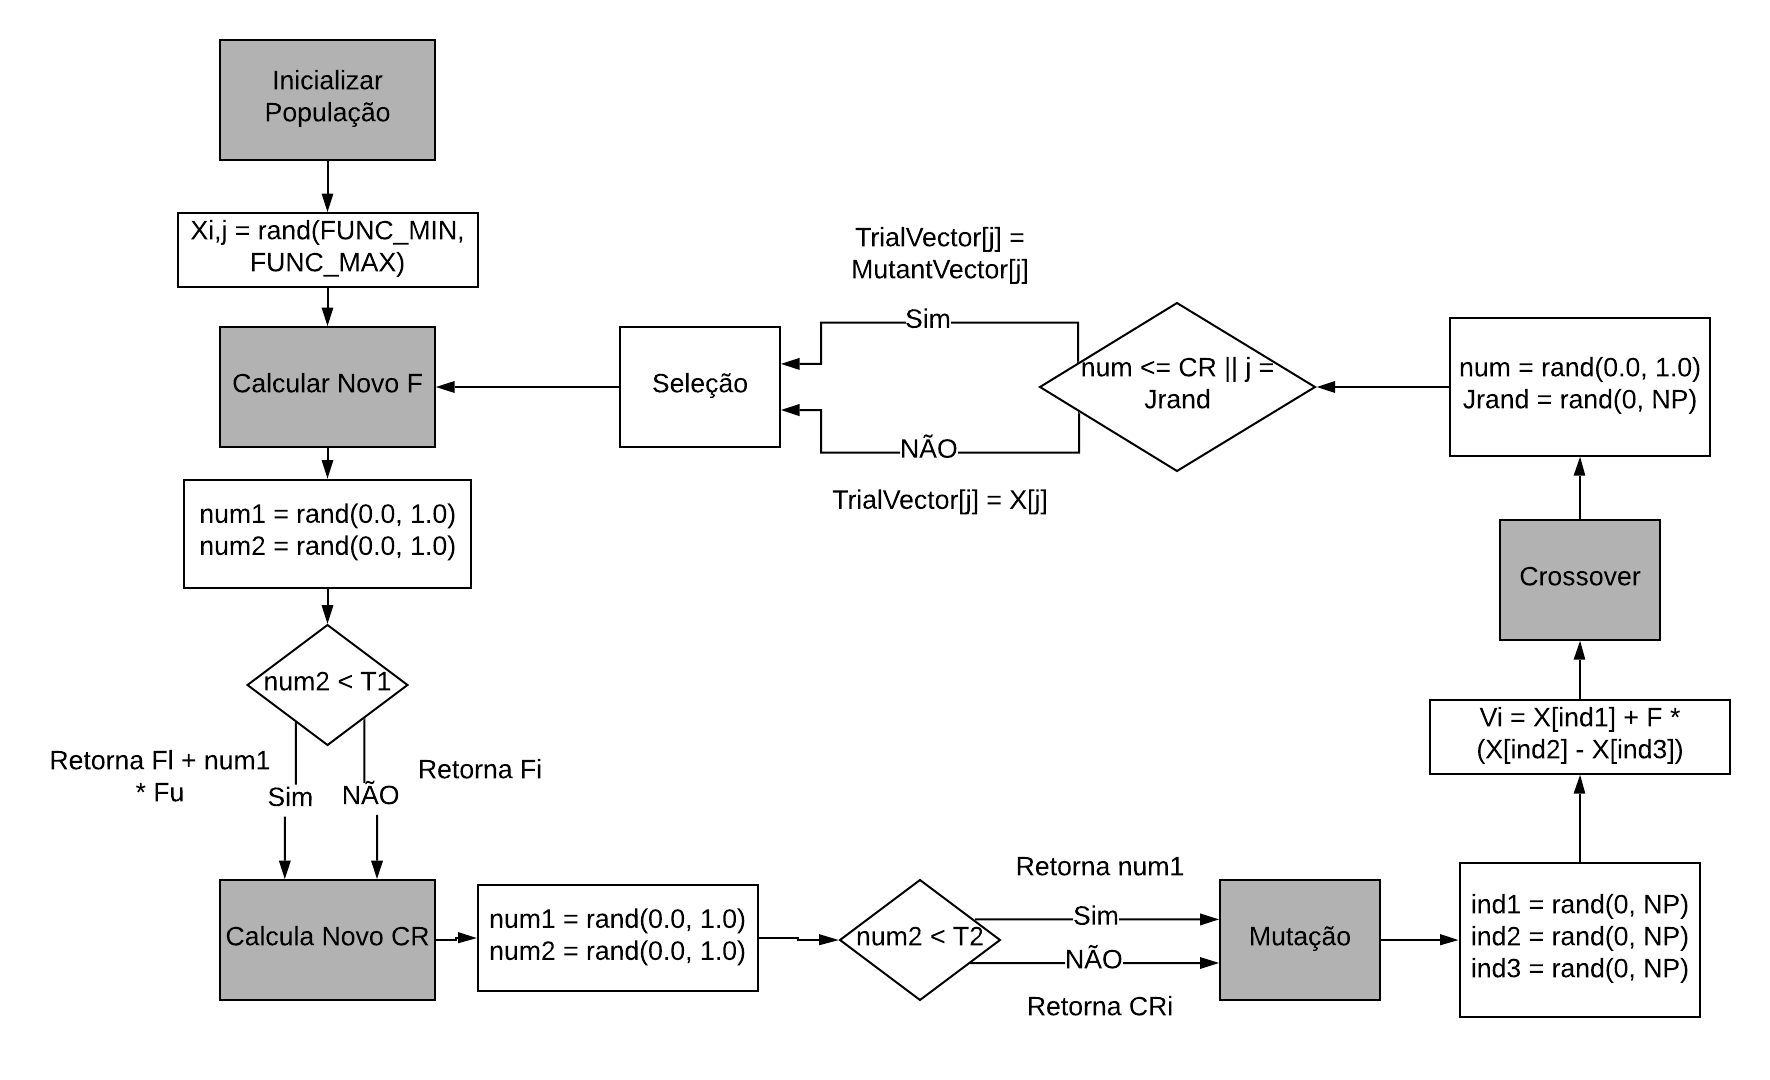
\includegraphics[width=0.9\linewidth]{figuras/Diagrama_de_Blocos.png}
    \captionof{figure}{Diagrama de Blocos do jDE}
    \label{fig:jDE}
}

\subsection{Algoritmo Seno e Cosseno}

O SCA (Sine Cosine Algorithm) cria múltiplas soluções randômicas iniciais e requer que as mesmas flutuem em direção ou na direção oposta da melhor solução usando um modelo matemático baseado nas funções seno e cosseno \cite{mirjalili}.

A seguinte equação de \textit{update} é utilizada para realizar as fases de intensificação e diversificação do algoritmo \cite{mirjalili}:

\begin{equation}
x_i^{t+1} = 
\begin{cases}
	x_i^t + r1 * seno(r2) * |r3 * p_i^t - x_i^t|    & \text{se $r4 < 0.5$}\\
    x_i^t + r1 * cosseno(r2) * |r3 * p_i^t - x_i^t| & \text{se $r4 \geq 0.5$}
\end{cases}
\end{equation}

Onde $p_i^t$ é o ponto de destino, ou seja, a melhor solução até então encontrada pelo algoritmo; e r1, r2, r3 e r4 são os quatro parâmetros do SCA \cite{mirjalili}:

\begin{itemize}
    \item r1 - parâmetro que faz o balanço entre intensificação e diversificação, mudando de forma auto-adaptativa o intervalo das funções seno e cosseno a partir da seguinte equação:
    \begin{equation}
        r1 = a - t * \frac{a}{T}
    \end{equation}
    Onde $t$ é a iteração atual; $T$ é a quantidade máxima de iterações; e $a$ é uma constante com o valor de 2;
    \item r2 - parâmetro randômico dentro do intervalo $[0, 2\pi]$ que define o quão grande deve ser o movimento em direção ou direção oposta ao ponto de destino;
    \item r3 - peso aleatório no intervalo $[0, 2]$ que estocasticamente enfatiza ($r3 > 1$) ou não ($r3 < 1$) o efeito do ponto de destino para calcular a distância do movimento;
    \item r4 - valor aleatório no intervalo $[0, 1]$ que faz a mudança entre seno e cosseno.
\end{itemize}

O SCA começa com um conjunto de soluções aleatórias, e então salva a melhor solução encontrada até o momento, a atribui ao ponto de destino e atualiza todas as outras soluções com respeito à ela \cite{mirjalili}. Ao mesmo tempo, os intervalos das funções seno e cosseno são atualizados enquanto o contador de iterações aumenta \cite{mirjalili}. O algoritmo termina quando o número máximo de iterações é alcançado ou quando uma certa acurácia do resultado é alcançada \cite{mirjalili}.

Como podemos observar no diagrama de blocos da figura \ref{fig:SCA}, existem dois pontos no algoritmo que utiliza-se a randomização. O primeiro é ao iniciar os indivíduos da população no espaço de busca; e o segundo é ao atualizar os parâmetros r2, r3 e r4 do SCA. Para realizar essa randomização, o algoritmo por padrão utiliza a distribuição uniforme.

{
    \centering
    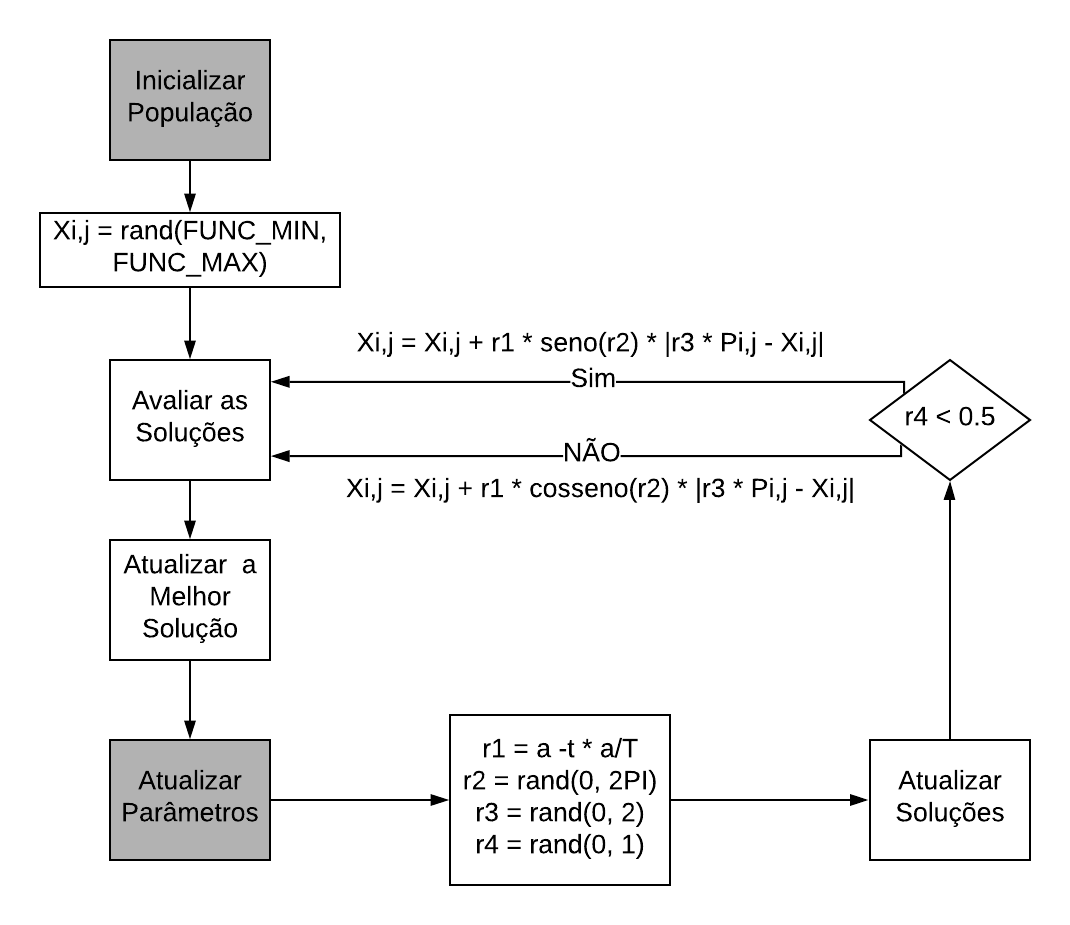
\includegraphics[width=0.7\linewidth]{figuras/Diagrama_SCA.png}
    \captionof{figure}{Diagrama de Blocos do SCA}
    \label{fig:SCA}
}

\section{Problemas do Mundo Real e Funções Benchmark}

Em geral, problemas sem restrições podem ser classificados em duas categorias: funções de teste, ou funções \textit{benchmark}, e problemas do mundo real \cite{jamil}. As funções de teste são problemas artificiais e podem ser usadas para avaliar o comportamento de um algoritmo em situações diversas e difíceis \cite{jamil}. Os problemas artificiais podem incluir mínimos globais únicos, únicos ou múltiplos mínimos globais na presença de muitos mínimos locais, vales longos e estreitos, efeitos de espaço nulo e superfícies planas \cite{jamil}. Esses problemas podem ser facilmente manipulados e modificados para testar os algoritmos em diversos cenários \cite{jamil}. Alguns exemplos de funções \textit{benchmark} são as funções Schaffer, Rastrigin, Griewank e Rosenbrock. 

Por outro lado, os problemas do mundo real se originam de campos diferentes como física, química, engenharia, matemática, entre outros \cite{jamil}. Esses problemas são difíceis de manipular e podem conter expressões algébricas ou diferenciais complicadas e podem exigir uma quantidade significativa de dados para compilar \cite{jamil}. 

\chapter{Revisão da Literatura} \label{chap2}

\section{Grey Wolf Optimizer com Mapa Caótico}

De acordo com o teorema No Free Lunch (NFL), nenhuma metaheurística é adequada para todas as aplicações existentes \cite{saxena}. Sendo assim, é sempre necessário que algumas modificações sejam incorporadas para fazer com que uma metaherística se torne adequada para uma aplicação em particular \cite{saxena}. Além disso, sequências caóticas são símbolos de aleatoriedade e comportamento barulhento - por isso, muitos algoritmos de otimização têm utilizado essas sequências caóticas ao invés de Passeios Aleatórios (geração de números aleatórios), pelo fato de que os passeios aleatórios nem sempre implementam a busca global muito bem \cite{saxena}.

Com essa motivação, o trabalho de \cite{saxena} propõe uma nova variante do algoritmo Grey Wolf Optimizer (GWO), o $\beta$-GWO. Este trabalho adapta o algoritmo original, que é baseado na hierarquia de liderança e nas estratégias de caça dos lobos cinza \cite{saxena}. Os lobos cinza vivem em matilhas divididas em quatro categorias: Alpha, Beta, Omega e Delta \cite{saxena}. Os principais passos do algoritmo envolvem circular a presa; caçar a presa e atacar a presa, fase responsável pela intensificação do algoritmo que é realizada pelo decremento linear do vetor de controle $\Vec{a}$ (2 até 0) \cite{saxena}. O decremento deste parâmetro permite que os lobos cinza ataquem a presa enquanto ela para de se mover \cite{saxena}.

A adaptação feita foi mudar o vetor de controle $\Vec{a}$ caoticamente de forma que a diversificação do espaço de busca possa se manter viva até os últimos passos das iterações \cite{saxena}. Baseado nas observações feitas ao longo do trabalho, os autores concluíram que incorporar caos no mecanismo de mudança entre as fases de diversificação e intensificação melhora esse mecanismo \cite{saxena}. Além disso, habilita os agentes de busca com uma melhor capacidade de intensificação e diversificação até a última iteração e, também aumenta a velocidade de busca após a fase de diversificação, que resulta em melhores características de convergência \cite{saxena}.

\section{Análise de Paisagem de Fitness Usando um Algoritmo de Passeio Aleatório Baseado em Caos}

A complexidade de um problema e a habilidade de uma técnica de busca heurística para obter a solução ótima pode ser determinada usando uma \textit{Fitness Landscape Analysis} (FLA) ou uma análise de paisagem de aptidão \cite{jana}. Uma paisagem pode ser interpretada como uma superfície no espaço de busca que define o \textit{fitness} de cada solução potencial \cite{jana}. FLA é um método que detecta e destaca características salientes de um problema de otimização, como a robustez, modalidade, decepção, presença de funis, suavidade, neutralidade e separabilidade de variáveis \cite{jana}.

Um \textit{Random Walk} (RW) ou passeio aleatório é uma formalização matemática de um caminho consistindo em passos aleatórios sucessivos \cite{jana}. Algoritmos RW foram desenvolvidos para capturar uma sequência de interação vizinha de pontos de amostra sobre o espaço de busca, sem usar nenhuma informação sobre o \textit{fitness} do problema de otimização \cite{jana}. O passeio aleatório simples é construído através da amostragem de um ponto inicial $X_1$ aleatoriamente, e depois gerando os próximos pontos $X_2 ... X_n$ até que um número pré-definido de pontos $N$ na vizinhança seja alcançado \cite{jana}.

Sendo assim, o trabalho de \cite{jana} propõe o algoritmo Chaotic Random Walk (CRW) em espaços de busca contínuos para obter a estrutura da paisagem para determinar as características de um problema. CRW é um resultado baseado na inspiração do comportamento caótico em conexão com a geração determinística de números pseudo-aleatórios \cite{jana}. A ideia é utilizar esses números pseudo-aleatórios dados por um mapa caótico para gerar pontos de amostra para o RW \cite{jana}. Esses números pseudo-aleatórios controlam o tamanho dos passos e determinam a direção do algoritmo proposto \cite{jana}.

Em Teoria do Caos, mapas caóticos são usados para gerar sequências de números pseudo-aleatórios conhecidos como números caóticos pseudo-aleatórios \cite{jana}. Alguns exemplos são o mapa Logístico, mapa de Tent, mapa de Chebyshev, mapa Cúbico e mapa ICMIC \cite{jana}.

Como resultado, o trabalho de \cite{jana} mostra que a distribuição dos pontos de amostra do CRW sobre o espaço de busca é mais uniforme que a distribuição do algoritmo Random Walk simples, e consequentemente, providencia uma melhor cobertura de toda a área do espaço de busca \cite{jana}.

\section{Evolução Diferencial e Séries Caóticas}

Pesquisas recentes em abordagens caóticas para meta-heurísticas usam vários mapas caóticos no lugar de geradores de números pseudo-aleatórios (PRNGs) \cite{senkerik}. Essa abordagem caótica não convencional está fortemente ligada com a importância da randomização dentro das heurísticas como compensação por um número limitado de movimentos de busca \cite{senkerik}. Caos com as suas propriedades como ergodicidade, estocasticidade, auto-similaridade e densidade das órbitas periódicas se tornou bastante popular e uma ferramenta moderna para melhorar o desempenho de várias técnicas computacionais evolucionárias (ECTs) \cite{senkerik}.

Mesmo assim, as perguntas se mantém, quanto ao por que ele funciona, e porque pode ser um benefício utilizar sequências caóticas para números pseudo-aleatórios dirigindo a seleção, mutação, crossover e outros processos \cite{senkerik}. Sendo assim, o trabalho de \cite{senkerik} é destinado a analisar a influência das sequências caóticas no desempenho de quatro variantes da Evolução Diferencial (DE): os esquemas de mutação do DE original DE/Rand/1 e DE/Best/1; jDE; e SHADE.

A ideia geral é substituir o PRNG padrão com um sistema caótico; e no trabalho de \cite{senkerik}, nove sistemas foram utilizados: mapa Arnold Cat; mapa Burgers; Logístico Atrasado; mapa Padrão Dissipativo; mapa Hénon; mapa Ikeda; mapa Lozi; mapa Sinai; e mapa Tinkerbell. De maneira geral, as versões caóticas aparentam ser muito eficientes para encontrar os valores mínimos da função objetivo \cite{senkerik}. Além disso, o desempenho do comparado DE original e suas variantes caóticas foi similar, ou em alguns casos, as versões caóticas foram significamente piores \cite{senkerik}.



\chapter{Resultados Parciais} \label{cap3}
